\documentclass[12pt]{article}%
\usepackage{amsfonts}
\usepackage{fancyhdr}
\usepackage{comment}
\usepackage[a4paper, top=2.5cm, bottom=2.5cm, left=2.2cm, right=2.2cm]%
{geometry}
\usepackage{times}
\usepackage{amsmath}
\usepackage{changepage}
\usepackage{stfloats}
\usepackage{amssymb}
\usepackage{graphicx}
\usepackage{indentfirst}

\setlength{\parindent}{2em}
\setcounter{MaxMatrixCols}{30}
\newtheorem{theorem}{Theorem}
\newtheorem{acknowledgement}[theorem]{Acknowledgement}
\newtheorem{algorithm}[theorem]{Algorithm}
\newtheorem{axiom}{Axiom}
\newtheorem{case}[theorem]{Case}
\newtheorem{claim}[theorem]{Claim}
\newtheorem{conclusion}[theorem]{Conclusion}
\newtheorem{condition}[theorem]{Condition}
\newtheorem{conjecture}[theorem]{Conjecture}
\newtheorem{corollary}[theorem]{Corollary}
\newtheorem{criterion}[theorem]{Criterion}
\newtheorem{definition}[theorem]{Definition}
\newtheorem{example}[theorem]{Example}
\newtheorem{exercise}[theorem]{Exercise}
\newtheorem{lemma}[theorem]{Lemma}
\newtheorem{notation}[theorem]{Notation}
\newtheorem{problem}[theorem]{Problem}
\newtheorem{proposition}[theorem]{Proposition}
\newtheorem{remark}[theorem]{Remark}
\newtheorem{solution}[theorem]{Solution}
\newtheorem{summary}[theorem]{Summary}
\newenvironment{proof}[1][Proof]{\textbf{#1.} }{\ \rule{0.5em}{0.5em}}

\usepackage{mathtools}

\newcommand{\Q}{\mathbb{Q}}
\newcommand{\R}{\mathbb{R}}
\newcommand{\C}{\mathbb{C}}
\newcommand{\Z}{\mathbb{Z}}

\begin{document}

\title{MATH2040C Homework 6}
\author{ZHENG Weijia (William, 1155124322)}
\date{April 9, 2021}
\maketitle



\section{Section 6.1, Q8}

\begin{figure}[htp]
    \centering % 图片居中
    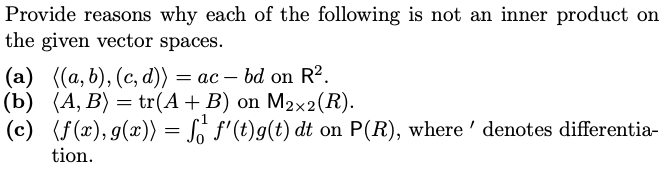
\includegraphics[width = 16cm]{img/Q1.png}
    %\caption{Section 6.1 Q8}
    %\label{fig:figure1label}
\end{figure}

\subsection{(a)}
Suppose this is an inner product. Then $\langle\, x,x \rangle \geq 0$ should hold $\forall x \in \mathbb{R}^2.$

Let $x=(1,10).$ Then $\langle\, x,x \rangle=\langle\, (1,10),(1,10) \rangle=1^2-10^2=-99<0.$

Therefore, this is not an inner product.

\subsection{(b)}
Suppose this is an inner product. Then $\langle\, x,x \rangle \geq 0$ should hold $\forall x \in M_{2\times 2}(R).$

Let $x=\begin{pmatrix} -1&0\\0&-1\end{pmatrix}$. Then $$\langle\, x,x \rangle=tr(x+x)=-2-2=-4<0.$$

Therefore, this is not an inner product.

\subsection{(c)}
Suppose this is an inner product. Then $\forall f,g \in P(\mathbb{R}), \overline{\langle\, g,f \rangle}=\langle\, f,g \rangle$ should hold.

Let $f(x)=x, g(x)=x^2+x.$

Then $$\langle\, f,g \rangle=\int_{0}^{1} 1(x^2+x) \,dx=\frac{5}{6}.$$

$$\overline{\langle\, g,f \rangle}=\overline{\int_{0}^{1} (2x+1)x \,dx}=\frac{7}{6}.$$

Therefore $\overline{\langle\, g,f \rangle} \neq \langle\, f,g \rangle$ for some $f,g \in P(\mathbb{R}).$

Hence, this is not an inner product.

Done.

\noindent\rule[0.1ex]{\linewidth}{1pt}

\section{Section 6.1, Q17}
\begin{figure}[htp]
    %\centering % 图片居中
    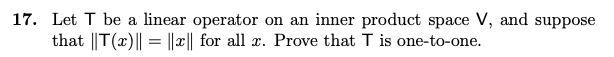
\includegraphics[width = 15cm]{img/Q2.png}
    %\caption{Section 6.1 Q17}
    %\label{fig:figure1label}
\end{figure}

Note that because we have $||T(x)||=||x||.$ Then $\forall x\in V$, with $x\neq 0$ we have $$||T(x)||=||x||>0.$$

Therefore $x\neq 0.$ 

Note that $||T(0)||=||0||=0$, which implies $$T(0)=0.$$

Hence $N(T)=\{0\}.$

Hence, $T$ is one-to-one.

Done.

\noindent\rule[0.1ex]{\linewidth}{1pt}


\section{Section 6.1, Q18}
\begin{figure}[htp]
    %\centering % 图片居中
    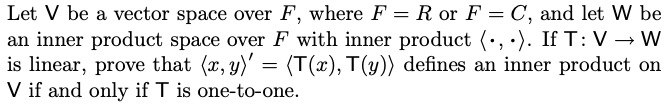
\includegraphics[width = 15cm]{img/Q3.png}
\end{figure}

\subsection{If part}
In the if part, we assume $T$ is one-to-one and try to prove $\langle\, \cdot , \cdot \rangle^{'}$ is an inner product.

One-to-one implies $N(T)=\{0\}.$ Then $\forall x (\neq 0) \in V, T(x)\neq 0.$ Therefore $$\langle\, x, x \rangle^{'}=\langle\, T(x) , T(x) \rangle>0.$$
Because $\langle\, \cdot , \cdot \rangle$ is an inner product.

Also note that $\forall x,y,z \in V, \forall c \in F,$ $$\langle\, x+z , y \rangle^{'}=\langle\, T(x+z) , T(y) \rangle=\langle\, T(x)+T(z) , T(y) \rangle=\langle\, T(x) , T(y) \rangle + \langle\, T(z) , T(y) \rangle$$

$$=\langle\,x , y \rangle^{'} + \langle\, z , y \rangle^{'}.$$

Besides, $$\langle\, cx , y \rangle^{'}=\langle\, T(cx) , T(y) \rangle=\langle\, cT(x) , T(y) \rangle=c\langle\, T(x) , T(y) \rangle=c\langle\, x , y \rangle^{'}.$$

And finally, $$\overline{\langle\, x , y \rangle^{'}}=\overline{\langle\, T(x) , T(y) \rangle}=\langle\, T(y) , T(x) \rangle=\langle\, y , x \rangle^{'}.$$

Based on all above, $\langle\, \cdot , \cdot \rangle^{'}$ is an inner product.

\subsection{Only if part}
In the only if part, we have $\langle\, \cdot , \cdot \rangle^{'}$ is already an inner product and try to prove $T$ is injective.

Note that $T$ is linear, then $T(0)=0$ must hold.

Becasue $\forall x(\neq 0)\in V, \langle\, x , x \rangle^{'}=\langle\, T(x), T(x) \rangle>0.$ Therefore $\forall x\neq 0, T(x)\neq 0.$ 

Therefore $N(T)=\{0\},$ follows that $T$ is injective.

Done.

\noindent\rule[0.1ex]{\linewidth}{1pt}

\section{Section 6.1, Q19}
\begin{figure}[htp]
    %\centering % 图片居中
    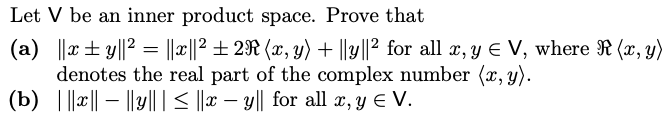
\includegraphics[width = 15cm]{img/Q4.png}
\end{figure}

\subsection{(a)}
Our goal is to prove $ 2\mathcal{R}\langle\,x,y\rangle=||x+ y||^2-||x||^2-||y||^2$ and $ -2\mathcal{R}\langle\,x,y\rangle=||x-y||^2-||x||^2-||y||^2.$

For the plus sign, note that the $$R.H.S.=\mathcal{R}\langle\,x + y,x + y\rangle-\mathcal{R}\langle\,x,x\rangle-\mathcal{R}\langle\,y,y\rangle$$

$$=\mathcal{R}\langle\,x,y\rangle+\mathcal{R}\langle\,y,x\rangle.$$

Note that $\mathcal{R}\langle\,x,y\rangle = \mathcal{R}\langle\,y,x\rangle$ because $\overline{\langle\,x,y\rangle}=\langle\,y,x\rangle.$

Therefore $L.H.S.=R.H.S..$

For the minus sign, note that the $$R.H.S.=\mathcal{R}\langle\,x - y,x - y\rangle-\mathcal{R}\langle\,x,x\rangle-\mathcal{R}\langle\,y,y\rangle$$

$$=\mathcal{R}\langle\,x,-y\rangle+\mathcal{R}\langle\,-y,x\rangle.$$ 

Which is equal to $2\mathcal{R}\langle\,x,-y\rangle=-2\mathcal{R}\langle\,x,y\rangle=L.H.S..$

Therefore, (a) is proved. Done.

\subsection{(b)}
To prove (b), it is suffice to prove $|~||x||-||y||~|^2\leq ||x-y||^2.$

Iff, $$||x||^2+||y||^2-2||x|| \cdot ||y||\leq ||x||^2 + 2\mathcal{R}\langle\,x,y\rangle+||y||^2.$$

iff, $$||x||\cdot ||y||\geq \mathcal{R}\langle\,x,y\rangle.$$

Which is bound to be true because $$||x||\cdot ||y||\geq |\langle\,x,y\rangle|\geq \mathcal{R}\langle\,x,y\rangle.$$

Done.

\noindent\rule[0.1ex]{\linewidth}{1pt}

\section{Section 6.1, Q23}

\begin{figure}[htp]
    %\centering % 图片居中
    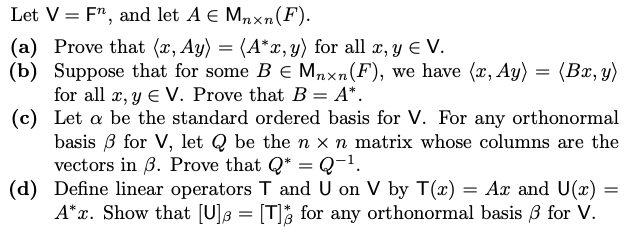
\includegraphics[width = 15cm]{img/Q5.png}
\end{figure}

\subsection{(a)}
Denote $T=L_{A}:V \to V,$ note that $T$ is linear. Note that we have a corollary that $(L_{A})^{*}=L_{A^{*}}.$

Then $\langle\,x,Ay\rangle=\langle\,A^{*}x,y\rangle$ follows. Done.

\subsection{(b)}
Let $\beta=\{v_1,v_2,\dots, v_n\}$ be a standard basis for $V=F^{n},$ then we have a expression of $A$ such that $\forall x \in V,$
$$B(x)=\sum_{i=1}^{n}\langle\,B(x),v_i\rangle v_i=\sum_{i=1}^{n}\langle\,x,Av_i\rangle v_i=\sum_{i=1}^{n}\langle\,A^{*}x,v_i\rangle v_i=A^{*}(x).$$

Therefore, $B=A^{*}.$

Done.

\subsection{(c)}




\end{document}
